\chapter{Návrh modelu}\label{chap:proposal}

V tejto kapitole si opíšeme cieľ diplomovej práce, zameriame sa na návrh modelu všetkých častí aplikácie a definujeme si požiadavky na ich funkcionalitu. 

Riešenie diplomovej práce bude pozostávať z dvoch hlavných častí. Prvou časťou bude navrhnutie synchronizačného servera, ktorý bude zabezpečovať výmenu informácií medzi klientmi. V druhej časti navrhneme samotný grafický editor obrázkov, vysvetlíme si spôsob integrácie editora do systému MediaWiki a popíšeme si jeho požadované vlastnosti.

\section{Cieľ práce}
\begin{itemize}
	\item Navrhnúť prostredie grafického editora.
	\item Implementovať grafický editor do prostredia MediaWiki pomocou rozšírenia.
	\item Navrhnúť a implementovať spôsob ukladania verzií výstupných súborov grafického editora.
	\item Navrhnúť a implementovat komunikačný protokol na synchronizáciu grafického editora pre viacero nezávislých používateľov.
	\item Integrovať rozšírenie s webovou stránkou fakulty http://wiki.matfyz.sk.
\end{itemize}

\section{Synchronizačný server}\label{sec:poziadavky_na_server}
Synchronizačný server bude pozostávať z aplikácie naprogramovanej v jazyku JavaScript. Spúšťaný bude v runtime prostredí NodeJS. Primárnou úlohou bude zaradiť pripojeného používateľa do miestnosti zodpovedajúcej editovanému súboru, vďaka čomu zabezpečíme synchronizáciu údajov medzi všetkými používateľmi pracujúcimi s týmto súborom. Využijeme pri tom knižnicu Socket.IO, konkrétne jej serverovú verziu, ktorá bude slúžiť ako hlavný komunikačný protokol postavený na báze WebSocket protokolu. Aplikácia synchronizačného servera bude pozostávať z niekoľkých entít (objektov), ktoré si postupne popíšeme v ďalších častiach tejto diplomovej práce.

\subsection{Popis entít synchronizačného servera}
\subsubsection{Entita používateľ}

Základnou entitou bude objekt \textit{Používateľ}, ktorý definuje vlastnosti pripojeného používateľa. Medzi informácie uchovávané v tomto objekte budú patriť \textit{meno}, jeho zodpovedajúca \textit{farba} kurzora, pod ktorou bude rýchlo rozpoznateľný inými používateľmi a \textit{jedinečný identifikátor} získaný po pripojení na server.

\subsubsection{Entita správa}
Editor poskytne možnosť textovej komunikácie medzi používateľmi. Kvôli tomu je potrebné navrhnúť objekt reprezentujúci takúto správu. Medzi jeho vlastnosti bude patriť informácia, kto správu odoslal, pre koho je určená, čas kedy bola odoslaná a taktiež textový obsah správy. Pre potreby lepšej informovanosti o stave pripojených používateľov je možné odosielať takzvanú systémovú správu, určenú pre všetkých používateľov.

\subsubsection{Entita objekt}
Informácie o objektoch grafickej plochy budú synchronizované pomocou JavaScriptového objektu typu \textit{Object}. Je to objekt dynamickej štruktúry s niekoľkými základnými vlastnosťami. Tými sú \textit{jedinečný identifikátor objektu}, informácia o \textit{stave uzamknutia} a v prípade uzamknutého objektu taktiež informácia o \textit{používateľovi, ktorý daný objekt uzamkol}. Ďalšie informácie o objekte sú závislé od jeho dátového typu generovaného na klientskej strane grafického editora.

\subsubsection{Entita miestnosť}
Každý používateľ bude po pripojení na synchronizačný server automaticky zaradený do miestnosti zodpovedajúcej editovanému súboru. Táto miestnosť bude reprezentovaná objektom Room s vlastnosťami popisujúcimi jej aktuálny stav. Bude sa tu nachádzať zoznam pripojených používateľov, zoznam odoslaných správ, zoznam grafických objektov editora, informáciu o formáte editovaného súboru a vlastnostiach grafickej plochy.

\subsubsection{Entita správca miestností}
Aby sa predišlo zbytočnému udržiavaniu stavov miestností, v ktorých sa nenachádzajú žiadni používatelia, musíme navrhnúť entitu, ktorá bude riadiť dynamické vytváranie a odstraňovanie miestností. Pre tento účel vytvoríme objekt RoomManager, ktorý bude obsahovať zoznam všetkých miestností a funkcie na vytvorenie miestnosti pri pripojení prvého používateľa a jej vymazanie v prípade, že sa z nej odpojil posledný používateľ.

\subsection{Funkčné požiadavky synchronizačného servera}

\begin{itemize}
	\item \textbf{Pripojenie používateľa} - vytvorí sa entita typu \code{User} a nastavia sa mu vlastnosti na základe zaslaného dopytu. 
	
	\item \textbf{Overenie pripojeného používateľa} - po pripojení nového používateľa sa overuje správnosť bezpečnostného tokenu. Ak bezpečnostný token nie je správny, používateľ nebude mať umožnené pripojenie do zvolenej miestnosti.
	
	\item \textbf{Vytvorenie miestnosti} - v prípade, ak sa pripojený používateľ má zaradiť do miestnosti, ktorá aktuálne neexistuje, takáto miestnosť je vytvorená a následne je do nej používateľ zaradený. V prípade, že daná miestnosť už vytvorená je, používateľ sa do nej zaradí automaticky a táto informácia sa odošle všetkým ostatným používateľom nachádzajúcim sa v miestnosti. S pripojením prvého používateľa je potrebné načítať informácie o editovanom obrazovom súbore. Docielime to HTTP dopytom na rozhranie API (\textbf{A}plication \textbf{P}rograming \textit{Interface}). Návratové hodnoty dopytu v prípade existujúceho súboru rozdelíme do príslušných vlastností aktuálnej miestnosti a následne ich odošleme formou odpovede pripájanému používateľovi.
	
	\item \textbf{Synchronizácia editora} - po pripojení a zaradení používateľa do miestnosti zodpovedajúcej editovanému súboru, bude server schopný prijímať synchronizačné správy o zmenách vykonaných používateľom v prostredí editora. 
	
	Pri \textit{vytvorení nového grafického objektu} editora sa odosiela požiadavka s informáciami o tomto objekte na synchronizačný server. Ten požiadavku spracuje, pridá objekt do zoznamu objektov na základe jeho jedinečného identifikátora a odošle informáciu o novom objekte všetkým ostatným používateľom pripojeným do miestnosti.
	
	S \textit{modifikáciou existujúceho grafického objektu} editora bude taktiež odoslaný dopyt o tejto akcii synchronizačnému serveru. Ten ho spracuje, zmení zodpovedajúci objekt na základe prijatých informácií a odošle správu o zmene objektu spolu so zmenenými údajmi všetkým ostatným používateľom.
	
	Ak je \textit{objekt v grafickom editore odstránený}, táto akcia bude taktiež odoslaná na synchronizačný server, spolu s jedinečným identifikátorom objektu. Ten ho spracuje, odstráni zodpovedajúci objekt zo zoznamu a následne odošle ostatným používateľom informáciu o jeho vymazaní.
	
	Aby sa predišlo konfliktom pri zmenách vlastností objektov, je potrebné navrhnúť proces ich automatického uzamykania. To zabezpečíme tak, že pri zvolení aktívneho objektu v grafickom editore bude odoslaná požiadavka na jeho uzamknutie daným používateľom na server. Táto akcia je znova synchronizovaná so zvyšnými editormi používateľov. V prípade že objekt už uzamknutý bol, odošle sa odpoveď o zamietnutí uzamknutia objektu.
	
	\item \textbf{Odpojenie používateľa} - pri tejto akcií je potrebné vykonať niekoľko úkonov. Najskôr musia byť odomknuté všetky objekty, ktoré boli uzamknuté odpájaným používateľom a následne sa odstráni z miestnosti. V prípade, že miestnosť zostane prázdna, vymaže sa. Inak je odoslaná informácia o odpojení používateľa všetkým zvyšným pripojeným klientom.
	
	\item \textbf{Odstránenie miestnosti} - ako sme spomenuli vyššie, miestnosť je automaticky odstránená pri odchode posledného používateľa. Tento proces zabezpečí entita \code{RoomManager}.
	
\end{itemize}

\section{Editor obrázkov}
Grafický editor implementujeme formou MediaWiki rozšírenia, naprogramovaného primárne v jazyku JavaSrcipt, s použitím frameworku AngularJS (kap.: \ref{sec:angular}). Na komunikáciu so synchronizačným serverom použijeme JavaScriptovú knižnicu Socket.IO (kap.: \ref{sec:socketio}), konkrétne jej klientskú verziu. Na vykresľovanie a udržiavanie stavu grafickej plochy použijeme knižnicu Fabric (kap.: \ref{sec:fabric}). 

\subsection{Funkčné požiadavky grafického editora}
\begin{itemize}
	\item \textbf{Otvorenie grafického editora} a v prípade upravovania existujúceho súboru jeho automatické načítanie.
	
	\item \textbf{Výber nástroja} - grafický editor poskytne viacero pracovných nástrojov, na vytváranie rôznych typov grafických objektov. Tie môžu byť zvolené kliknutím na tlačidlo reprezentujúce daný nástroj. 
	
	\item \textbf{Vytvorenie objektu} - po zvolení nástroja môžeme pridať do grafickej plochy nasledujúce objekty:
	\begin{itemize}
		\item \textbf{Obdĺžnik}, \textbf{elipsu}, \textbf{trojuholník}, \textbf{úsečku} a \textbf{textové pole} pomocou kliknutia na grafickú plochu a  ťahaním kurzora sa bude nastavovať ich veľkosť.
		\item \textbf{Polygón}, ktorého vrcholy sa budú pridávať postupným klikaním na grafickú plochu.
		\item \textbf{Obrázok} môže používateľ pridať zvolením nástroja na pridávanie obrázkov. Zobrazí sa ponuka na nahratie lokálneho súboru.
		\item \textbf{Voľne kreslená cesta} vytvorená kliknutím a ťahaním kurzora, s možnosťou nastavenia šírky a typu cesty, farby a veľkosti rozmazania.
	\end{itemize}
	
	\item \textbf{Výber aktívneho objektu / skupiny objektov} - používateľ vyberie aktívny objekt a následne sa zobrazí panel s možnosťou zmeny jeho vlastností.
	
	\item \textbf{Modifikácia vlastností aktívneho objektu} v závislosti od jeho typu. Základné vlastnosti ako výška, šírka, pozícia, uhol rotácie a skosenie možu byť nastavované pomocou transformácie obálky objektu. Tieto a ďalšie vlastnosti bude možné zmeniť aj pomocou zadávania hodnôt do zodpovedajúcich textových polí, prípadne tlačidlami a inými ovládacími prvkami.
	
	\item \textbf{Odstránenie objektu} z grafickej plochy. 
	
	\item \textbf{Zmena hĺbky} ovplyvňujúca prekrývanie jednotlivých objektov v grafickej ploche.
	
	\item \textbf{Lokálne uzamknutie} zamedzí používateľovi možnosť pohybu, rotácie, a zmeny veľkosti objektu.
	
	\item \textbf{Zmena viditeľnosti} - každý grafický objekt môže byť skrytý z grafickej plochy editora a následne znova zobrazený.
	
	\item \textbf{Kopírovanie, vystrihnutie, vloženie a duplikovanie} objektu.
	
	\item \textbf{Priblíženie grafickej plochy} - používateľ môže proporcionálne zväčšiť alebo zmenšiť grafickú plochu zmenou hodnoty skálovania(zoom).
	
	\item \textbf{Zmena vlastností grafickej plochy} - okrem skálovania môže používateľ nastaviť aj jej rozmery, od čoho sa odvíja veľkosť výsledného súboru a tým aj jeho kvalita a taktiež farbu pozadia. 
	
	\item \textbf{Zobrazenie zoznamu používateľov}
	
	\item \textbf{Režim celej obrazovky}, kedy sa skryjú ovládacie prvky systému MediaWiki a grafický editora sa zväčší na maximálnu dostupnú veľkosť okna internetového prehliadača používateľa.
	
	\item \textbf{Vycentrovanie grafickej plochy} na vertikálny a horizontálny stred okna grafického editora.
	
	\item \textbf{Chat} - používatelia si môžu vymieňať informácie formou krátkych textových správ. 
	
	\item \textbf{Uloženie revízie súboru} v systéme MediaWiki. 
	
	\item \textbf{Zatvorenie editora} a následné presmerovanie používateľa na stránku súboru.
\end{itemize}

\subsection{Integrácia do sytému MediaWiki}
Ako sme si opísali v časti \ref{sec:mediaWiki_extensions}, pre systém MediaWiki existuje viacero typov rozšírení. Pre naše riešenie sme si zvolili rozšírenie typu \textit{special page extension}. Učinili sme tak z dôvodu, že ide o najlepšiu voľbu z hľadiska vytvárania vlastného používateľského rozhrania a jeho špecifickej funkcionality. 

V systéme MediaWiki má každý multimediálny súbor svoju vlastnú podstránku. Aby sme používateľom umožnili otvoriť multimediálne súbory pomocou nášho editora, je potrebné integrovať tlačidlo na otvorenie súboru v editore. To umiestnime medzi tlačidlá hornej navigačnej lišty, kde sa nachádzajú odkazy na úpravu alebo vytvorenie stránky, zobrazenie histórie zmien, zmazanie, presunutie a zamknutie súboru. Používatelia môžu taktiež vytvoriť nový súbor, za pomoci odkazu na špeciálnu stránku editora. Keďže používateľ vytvára nový súbor, musí byť vyzvaný na zadanie jeho názvu. 

Systém MediaWiki umožňuje modifikovať položky hlavného menu a pridávať odkazy na rôzne stránky, vrátane špeciálnych stránok systému alebo rozšírení. Administrátor vďaka tomu môže jednoduchým spôsobom pridať odkaz na grafický editor do hlavného menu.

\subsection{Návrh ovládacích prvkov editora}
Väčšina prostredí grafických editorov, či už sú to vektorové, rastrové alebo 3D modelovacie editory využívajú rozdelenie ovládacích prvkov na 4 hlavné komponenty. Zoznam nástrojov zobrazený pri ľavom okraji okna editora, hlavné menu pri vrchnom a nastavenia nástrojov pri pravom okraji okna, s grafickou plochou uprostred týchto ovládacích komponentov. V našom prípade sme sa rozhodli použiť podobné rozloženie, kvôli zavedeným zvykom používateľov a tým pádom vyššej intuitívnosti pri používaní.

Rozloženie komponentov bude taktiež pozostávať zo 4. hlavných častí \refimg{obr:editorWireframeBase}:
\begin{itemize}
	\item \textbf{Panel nástrojov} s tlačidlami všetkých nástrojov a tlačidlami pre výber farby výplne a obtiahnutia objektu. V paneli sa taktiež nachádza tlačidlo na zapnutie prichytávania objektov k mriežke grafickej plochy.

	\item \textbf{Hlavný panel} obsahujúci tlačidlo na prepnutie zobrazenia do režimu celej obrazovky, tlačidlo na vycentrovanie grafickej plochy a rozbaľovací zoznam správ chatu. Okrem týchto tlačidiel tu nájdeme aj 3 rozbaľovacie (dropdown) tlačidlá \textit{Súbor}, \textit{Upraviť} a \textit{Objekt}. Rozbalením tlačidla \textit{Súbor} sa zobrazí ponuka na exportovanie grafickej plochy do viacerých formátov, uloženie revízie a zatvorenie editora. Po rozbalením tlačidla \textit{Upraviť} sa sprístupnia možnosti na kopírovanie, vystrihnutie, vloženie a duplikovanie objektu. Pod posledným tlačidlom \textit{Objekt}, sa zobrazia možnosti operácií s aktívnym objektom na zmenu hĺbky objektu v grafickej ploche.

	\item \textbf{Panel nastavení} tvorený dvoma komponentmi. Komponent vrstiev zobrazujúci zoznam všetkých grafických objektov s možnosťou ich rýchleho uzamknutia, skrytia. Vrstvy môžu byť preusporiadané pomocou ťahania, čím sa bude meniť ich hĺbka v grafickej ploche editora. Druhý komponent obsahujúci nastavenia aktuálneho kontextu editora bude dynamicky zobrazovať položky na nastavenie vlastností aktívneho objektu, grafickej plochy alebo nastavenia voľného kreslenia.

	\item \textbf{Grafická plocha}, v ktorej budú vykresľované jednotlivé grafické objekty.
\end{itemize}

Okrem týchto panelov je potrebné informovať používateľa o niektorých vykonávaných akciách formou vyskakovacích (\textit{popup}) správ, s možnosťou potvrdenia alebo prípadného zrušenia akcie. Obsah vyskakovacích okien je potrebné dynamicky vytvárať a modifikovať funkcionalitu potvrdzovacích tlačidiel.

\begin{figure}[h]
	\centerline{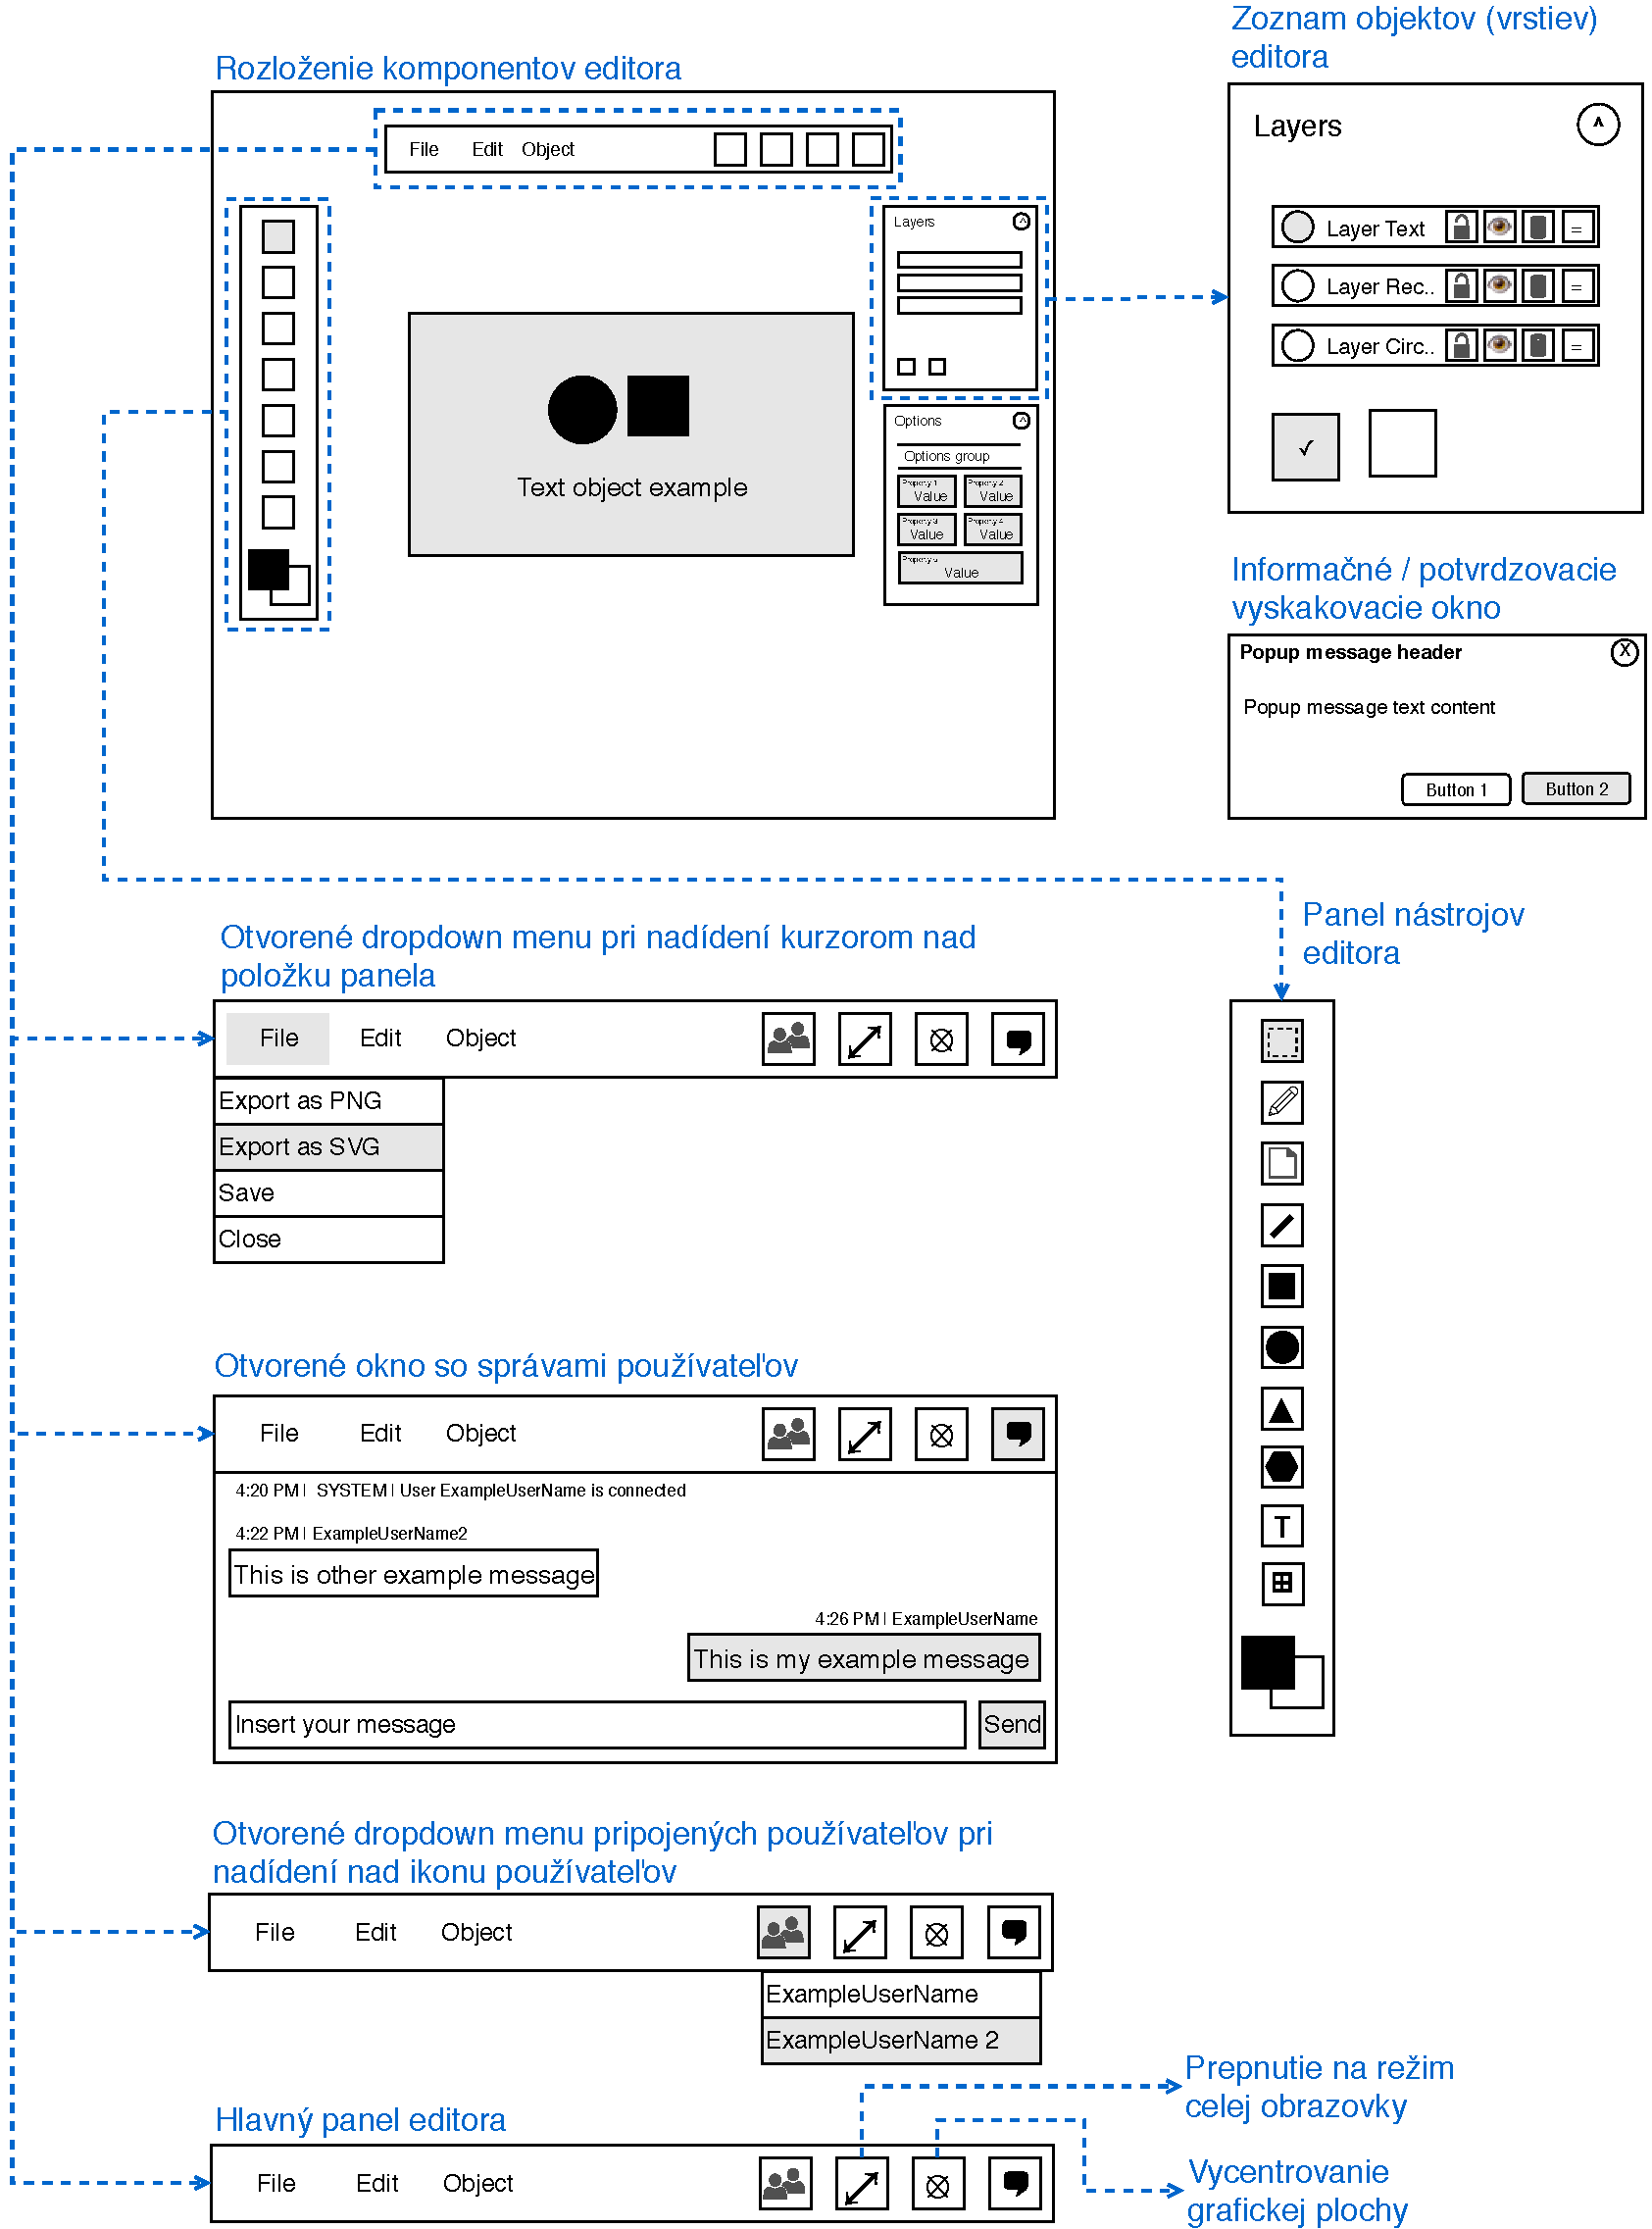
\includegraphics[width=1\textwidth]{images/diagrams/editor_wireframe_base}}
	\caption[Rozloženie komponentov editora]{Návrh rozloženia komponentov používateľského prostredia editora}
	\label{obr:editorWireframeBase}
\end{figure}
\FloatBarrier

